\appendix

\section{数据来源}

本文所使用的中文情感分析数据集来源于 HuggingFace 开源平台，由社区贡献者 \texttt{lansinuote} 整理发布。数据集名称：\texttt{lansinuote/ChnSentiCorp}。

\vspace{0.5em}
\noindent 数据集主页：\url{https://huggingface.co/datasets/lansinuote/ChnSentiCorp}

\vspace{1em}
\begin{figure}[htbp]
    \centering
    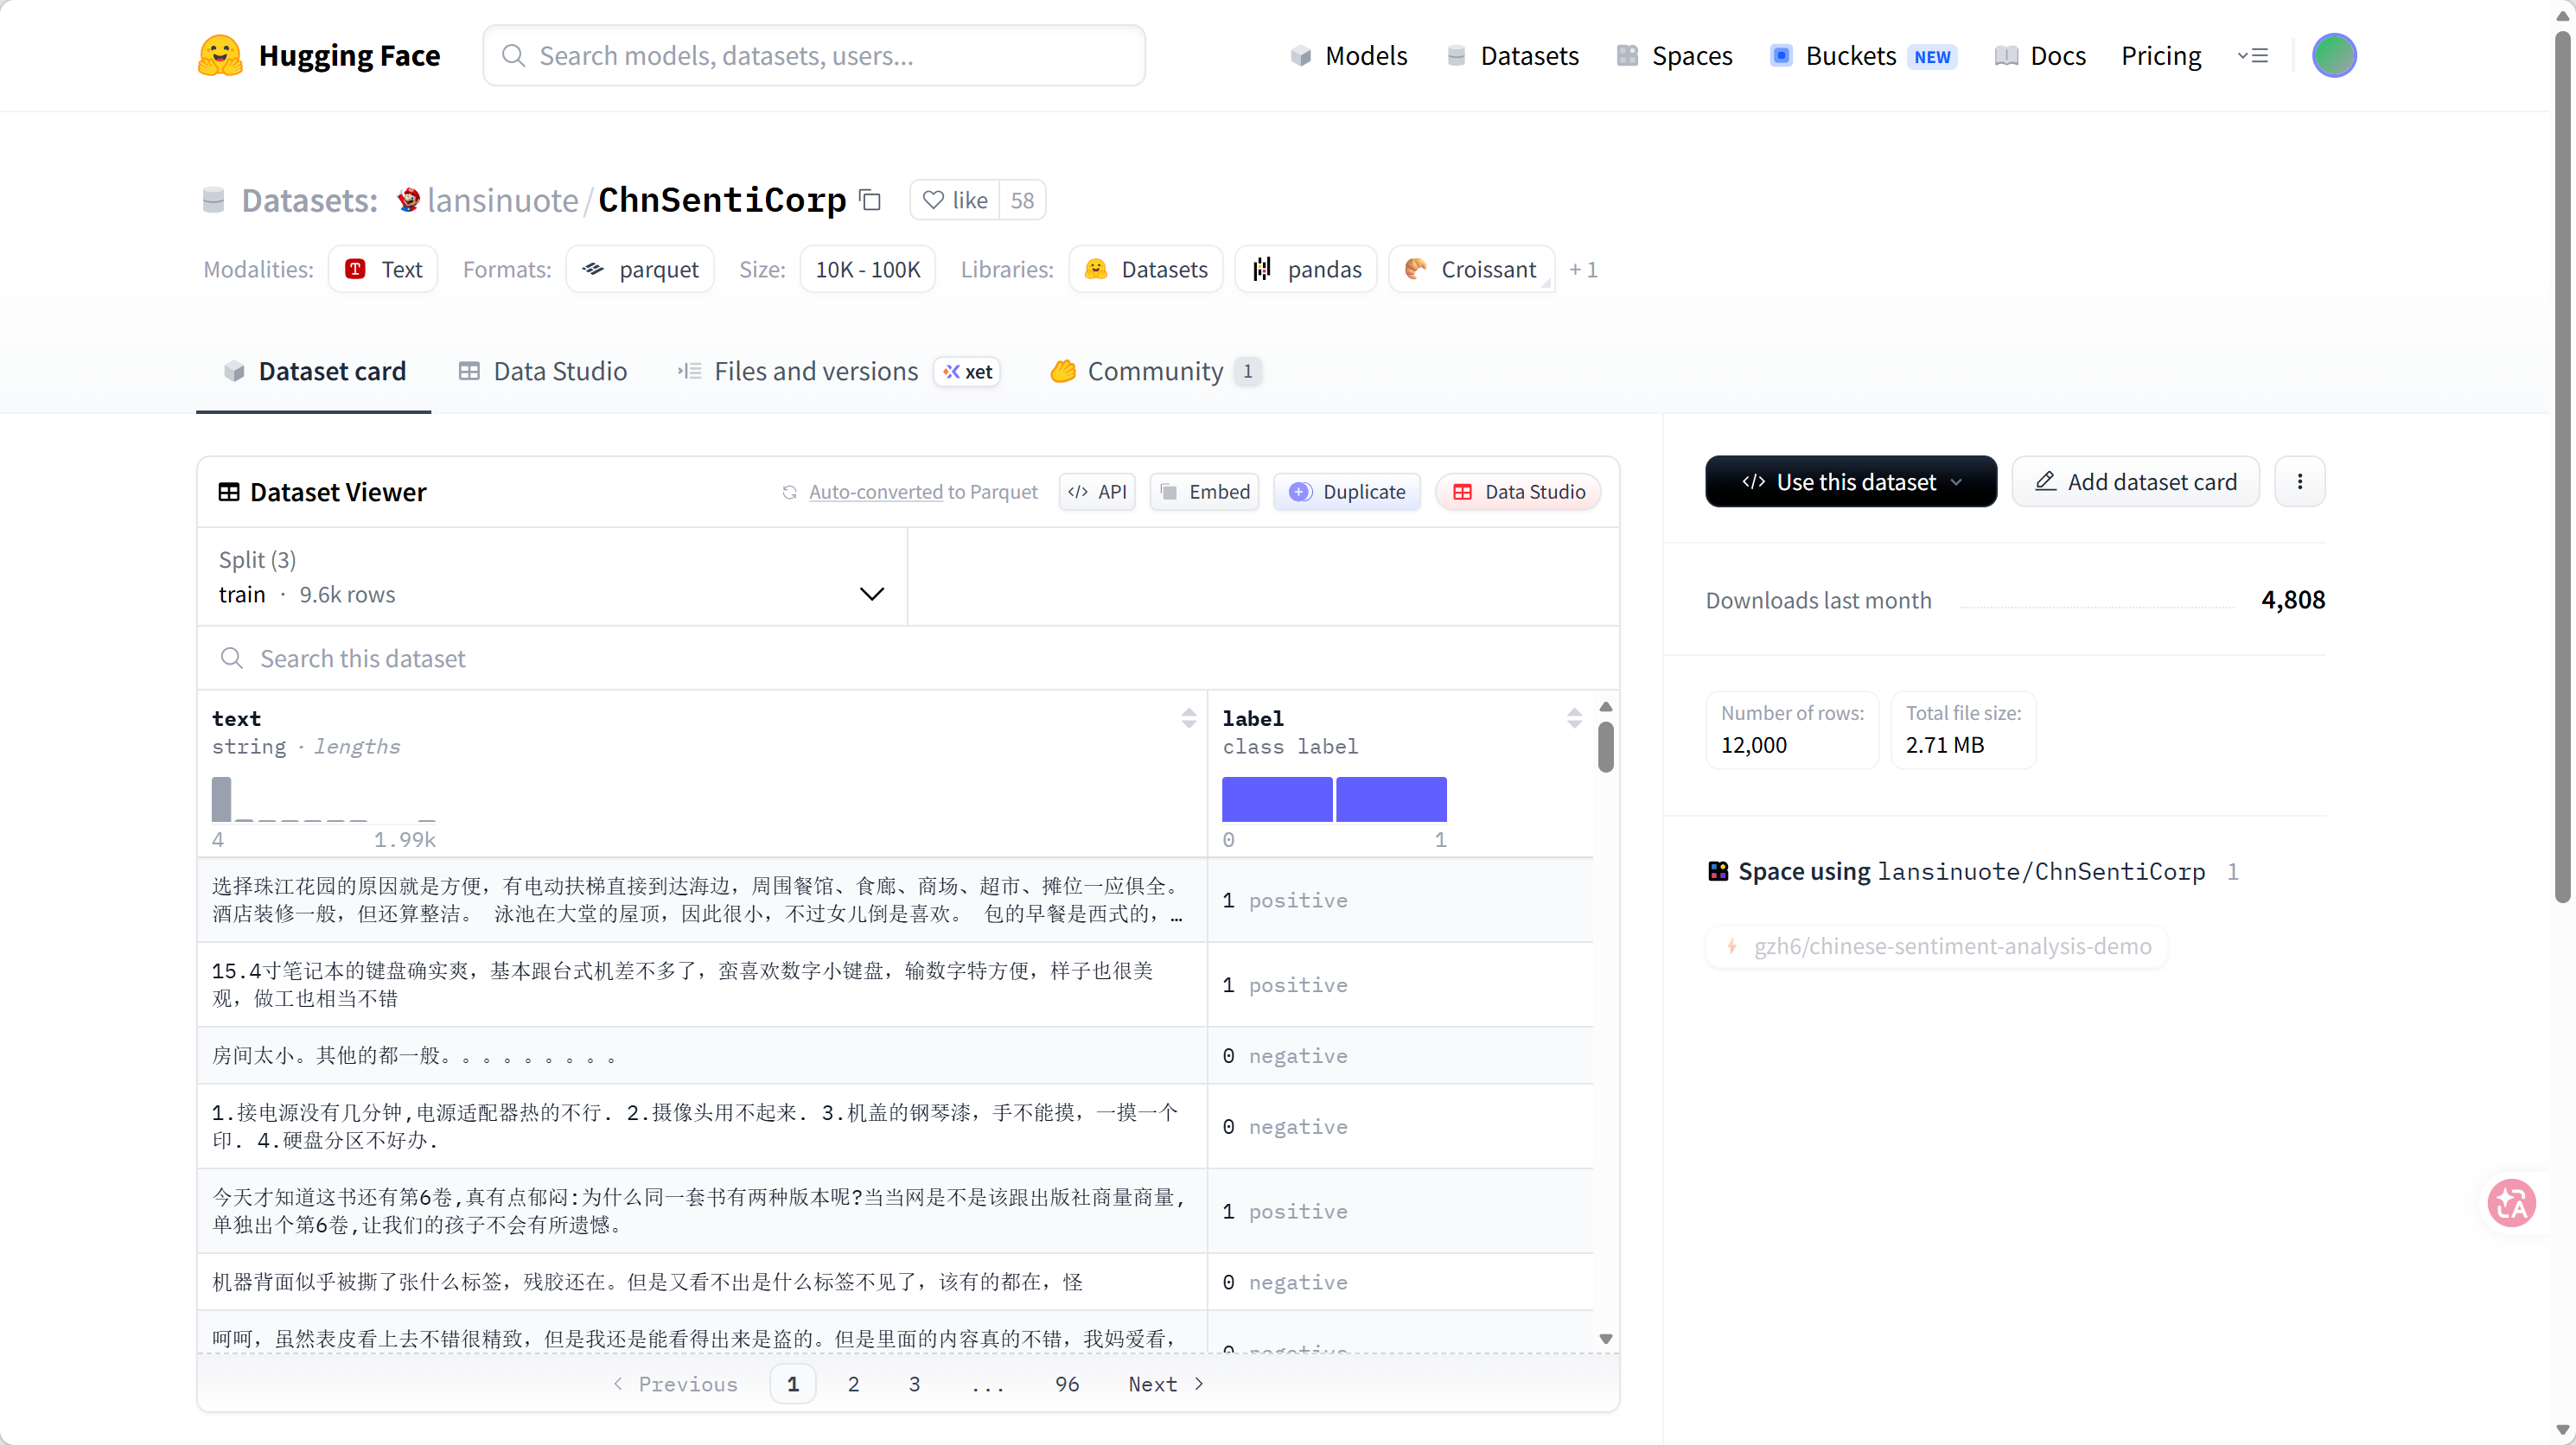
\includegraphics[width=0.92\textwidth]{数据来源截图.png}
    \caption{ChnSentiCorp 数据集 HuggingFace 页面截图}
    \label{fig:dataset_page}
\end{figure}

\section{实验代码}

本附录收录了本文全部五项实验及可视化绘图程序的完整 Python 源代码。所有代码均基于 PyTorch 2.11.0、Transformers 5.8.0、PEFT 0.19.1 及 Scikit-learn 1.8.0 编写，运行环境为 Ubuntu 22.04（Python 3.12，CUDA 12.8）。

代码文件包括：
\begin{enumerate}[nosep]
    \item \texttt{01\_svm.py}~——~SVM + TF-IDF 基线模型
    \item \texttt{02\_bilstm.py}~——~Bi-LSTM 序列分类模型
    \item \texttt{03\_bert.py}~——~BERT-base 预训练微调模型
    \item \texttt{04\_llm\_inference.py}~——~Qwen2.5-7B 零样本推理
    \item \texttt{05\_llm\_lora.py}~——~Qwen2.5-7B LoRA 微调模型
    \item \texttt{plot\_results.py}~——~论文图表可视化脚本
\end{enumerate}

各文件均已嵌入早停机制（Early Stopping），训练轮数与耗时记录均为实际实验结果。

\lstset{
    language=Python,
    basicstyle=\zihao{5}\ttfamily,
    keywordstyle=\color{blue},
    commentstyle=\color{gray}\itshape,
    stringstyle=\color{red!70!black},
    numbers=left,
    numberstyle=\tiny\color{gray},
    stepnumber=1,
    numbersep=8pt,
    frame=single,
    framesep=6pt,
    framerule=0.5pt,
    rulecolor=\color{gray!40},
    backgroundcolor=\color{gray!3},
    breaklines=true,
    breakautoindent=true,
    breakindent=2em,
    columns=flexible,
    keepspaces=true,
    tabsize=4,
    showstringspaces=false,
    captionpos=b,
    xleftmargin=1em,
    xrightmargin=1em,
    aboveskip=8pt,
    belowskip=8pt,
    abovecaptionskip=2pt,
    belowcaptionskip=2pt,
}

\subsection{SVM + TF-IDF 基线模型}

\lstinputlisting[caption={01\_svm.py — SVM + TF-IDF 基线模型}]{01_svm.py}

\subsection{Bi-LSTM 序列分类模型}

\lstinputlisting[caption={02\_bilstm.py — Bi-LSTM 序列分类模型}]{02_bilstm.py}

\subsection{BERT-base 预训练微调模型}

\lstinputlisting[caption={03\_bert.py — BERT-base 预训练微调模型}]{03_bert.py}

\subsection{Qwen2.5-7B 零样本推理}

\lstinputlisting[caption={04\_llm\_inference.py — Qwen2.5-7B 零样本推理}]{04_llm_inference.py}

\subsection{Qwen2.5-7B LoRA 微调模型}

\lstinputlisting[caption={05\_llm\_lora.py — Qwen2.5-7B LoRA 微调模型}]{05_llm_lora.py}

\subsection{论文图表可视化脚本}

\lstinputlisting[caption={plot\_results.py — 论文图表可视化脚本}]{plot_results.py}
